\documentclass[twocolumn,a4paper]{IEEEtranfr}
\usepackage[utf8]{inputenc}
\usepackage[utf8]{inputenc}
\usepackage{multicol}
\usepackage[french]{babel}
\usepackage[T1]{fontenc}
\usepackage{natbib}
\usepackage{verbatim}
\usepackage{graphicx}
\usepackage{url}
\usepackage[export]{adjustbox}
\usepackage[fleqn]{amsmath}
\usepackage{multicol}
\usepackage{lipsum}
\usepackage{placeins}
\usepackage{caption}

\title{Amélioration de l'ordonnancement des résultats dans un moteur de recherche}
\author{Baptiste \textsc{Aden}, Jordan \textsc{Bachelin}, Pierre-Henri \textsc{Collin}, Kévin \textsc{Ledy}, Haozhi \textsc{Li}}

\begin{document}

\maketitle

\begin{abstract}
L'objectif du projet est de démontrer l'efficacité d'une technologie de machine learning dans un moteur de recherche Apache Solr. Premièrement, nous avons appris à utiliser ce logiciel. Ensuite, nous avons généré nos propres données de test au format JSON qui est celui accepté par Solr. Puis, nous avons sélectionné une technologie de machine learning : Learning to Rank (LTR), plugin directement intégré au logiciel dans sa dernière version. Enfin, nous avons comparé les résultats de classement avec et sans le plugin. Ce dernier fournit de bons résultats et permet d'éviter une maintenance difficile de la pertinence du classement.
\end{abstract} 

\begin{keywords}
Moteur de recherche, classement et pertinence des résultats, machine learning, Big Data
\end{keywords}

\section{Introduction}
Face à de gros volumes de données, le classement des résultats a un rôle capital dans un moteur de recherche pour répondre aux attentes de l'utilisateur. De base dans Apache Solr, le score qu'obtient une requête (simple) est égale à la fréquence des termes de celle-ci dans l'ensemble de nos documents indexés\cite{docTFIDF}. Mais la plupart du temps, ce classement s'appuie également sur un ensemble de règles définies manuellement qui, si elles sont respectées par un document, celui-ci se verra attribué un score plus élevé et donc une meilleure place dans le classement. Pour que ce dernier reste pertinent, les administrateurs vont être amenés à ajouter des règles supplémentaires au cours du temps. À terme, cela devient difficile à maintenir car celles-ci peuvent entrer en conflit, ce qui peut entraîner de lourdes modifications pour un simple ajout.

L'objectif de notre projet consiste alors à mettre en place un prototype de moteur de recherche utilisant le "machine learning". Cette technologie a pour objectif d'améliorer et d'automatiser la pertinence de classement des résultats de recherches. Le but est de maîtriser cette technologie et de rendre compte à l'entreprise Jouve (notre client) de ses avantages et inconvénients. En fonction de notre retour, Jouve sera éventuellement amené à mettre en place le plugin pour améliorer son service client.

Dans cet article nous précisons dans un premier temps les problématiques auxquelles nous avons été confrontés et les méthodes employées pour y faire face, puis nous décrivons les résultats obtenus grâce à notre démarche, et nous concluons en apportant un point de vue critique sur l'ensemble du déroulement du projet.

\section{Méthodes, matériels et moyens}
Tout d'abord, c'est d'un commun accord que nous avons opté pour une méthode de travail agile, largement utilisée chez Jouve et très pratique dans le cas de ce projet. Le projet a été découpé en trois sprints :
\begin{itemize}
  \item \textbf{Sprint 1 - Familiarisation avec le projet :} au cours de cette phase nous avons installé Apache Solr, mis en place l'environnement général (GitHub, Google Drive, etc.) et surtout appris à utiliser Apache Solr. Ainsi, nous avons compris en quoi consistaient les règles de classement, en avons écrit quelques unes et avons créé nos propres données sur lesquelles travailler. Pour nous rapprocher au plus de l'utilisation qu'en fera Jouve, nous avons représenté une base de vêtements qui pourrait être celle d'un site e-commerce. Nous avons utilisé le format JSON (JavaScript Object Notation) pour créer nos différents vêtements (documents) de cette base. L'intérêt est double ici car ce type de données est parlant pour tout le monde et sera donc utile le jour de notre présentation orale. \textbf{[SCREEN CLOTHES.JSON TO CHANGE]}
  \begin{figure}[htpb]
    \begin{center}
        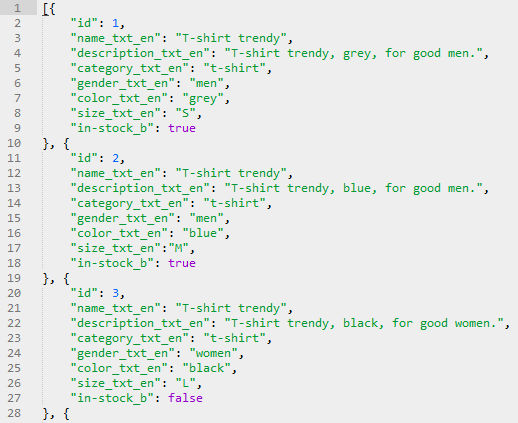
\includegraphics[width=7cm]{clothes.png}
    \end{center}
    \caption{Extrait de données JSON de vêtements}
    \label{clothes}
  \end{figure}
  
  \item \textbf{Sprint 2 - Comparaison d'algorithmes :} il s'agit du sprint principal. Initialement, la première tâche de ce sprint était de comparer LTR avec les outils présents dans Apache Solr en recherchant dans la littérature et en faisant l'expérience. En effet, bien que LTR soit dédié au réordonnancement de résultats, nous voulions nous assurer qu'il était rentable de l'utiliser : installation sans trop de complications, utilisation intuitive, documentation disponible, etc. Cependant, après la fin du sprint 1, une nouvelle version du logiciel est sorti, intégrant directement LTR et accompagné d'une documentation en ligne régulièrement mise à jour. Nous avons donc rapidement opté pour l'utilisation de ce plugin.\\
  La seconde tâche fut donc d'apprendre à utiliser LTR. Pour ce faire, nous avons utilisé la documentation en ligne ainsi que les exemples fournis pour réordonner des données selon de simples critères.\\
  
  \item \textbf{Sprint 3 - Finalisation :} Nous trouvions que la façon dont été affiché les résultats sur Apache Solr n'était pas très user-friendly. Nous avons donc durant ce sprint créé une petite application Web qui génère dans un premier temps ce qu'on appelle les "Training Data" permettant ensuite d'extraire un modèle LTR avec des poids différents sur les champs (sélectionnés dans notre feature) en fonction du jugement de l'utilisateur. Dans un second temps celui-ci permet de comparer le classement de résultats obtenus avant et après réordonnancement par ce dernier.\\
  Cinquante nouveaux documents ont également été créé afin de compléter notre base de départ et pour voir les différences quant aux résultats et scores obtenus sur nos différentes requêtes. Des statistiques ont été produite ensuite sur ces documents pour connaître le panel des types de vêtements, des tailles, des couleurs...etc que nous avions dans l'ensemble et ainsi mieux appréhender les scores que l'on obtenait avant d'utiliser Apache Solr avec le plugin LTR.\\
  A part cela, ce sprint a constitué principalement la partie "Livrables" de notre projet. En effet durant cette période, nous avons dû rendre compte auprès de nos tuteurs des résultats obtenus pour ce projet industriel. Il consistait donc notamment à la création de cet article scientifique mais également d'un poster reprenant ce qui est restitué ici mais de manière plus vulgarisée et concis cette fois-ci. Il fût très important pour celui-ci que l'objectif et les résultats de ce projet soit rapidement compris de tous (étudiants, professeurs, professionnels, intervenants, personnels...etc) car il est très probable que ce poster soit affiché et consulté dans le hall de notre école (École Supérieure d'Ingénieurs de Rennes) dans un futur proche.\\
\end{itemize}

Une réunion physique était planifiée toute les deux semaines chez Jouve afin de rendre compte à l'entreprise de l'avancement. Cela permettait d'alterner entre phase de familiarisation avec les technologies et phase de validation, car les encadrants professionnels ont une bonne connaissance d'Apache Solr.\\

À la différence d'un classement classique, LTR procède à un réordonnancement des résultats \textit{après} que la requête ait été faite et offre la possibilité de choisir le nombre d'éléments à classer. Cela permet de maintenir une latence faible sans perdre en pertinence de classement, car sur un gros volume de données, les utilisateurs ne parcourent que très rarement l'intégralité des résultats. 
Le plugin s'appuie sur divers éléments pour fonctionner : 
\begin{itemize}
  \item \textbf{Les "features"} sont l'équivalent des règles de classement de Solr. Elles définissent ce sur quoi le plugin doit se baser pour modifier le score d'un résultat.
  \item \textbf{Le "model"} liste un ensemble de features et attribue à chacune un poids qui servira au réordonnancement des résultats.
  \item \textbf{Les "training data"} sont des données diverses que l'on récupère (depuis une base de données par exemple) et qui vont permettre de générer les modèles décrits ci-dessus. Lors de cette génération, elles vont décider des poids à accorder à chaque feature grâce à un algorithme (nous utilisons RankSVM \cite{rankSVM}).
\end{itemize}




\section{Résultats}
Pour vérifier l'efficacité de LTR, nous avons comparé le classement des résultats lorsque l'on utilise uniquement Solr et lorsque l'on utilise LTR. Pour faciliter cette comparaison, nous avons développé une application web exploitant les données et les affichant dans deux tableaux côte à côte.
\\\\
\textbf{[SCREEN APP HAOZHI]}
\\\\
LTR marche + pas de maintenance manuelle

Mise en place + installation env dev; familiarisation Solr; création data perso; choix LTR; install + familiarisation LTR; comparaison résultats sans LTR/avec LTR;

\section{Analyse et discussion}
\textbf{[TODO]}

\section{Conclusion}
\textbf{[TODO]}



\bibliographystyle{unsrt}
\bibliography{ref}

\end{document}
